

\emph{Vaadin}~\cite{vaadin} es un \emph{framework} para el desarrollo de aplicaciones \emph{web} avanzadas, también conocidas como \emph{Rich-Internet Applications (RIA)}~\cite{ria}. El objetivo del paradigma \emph{RIA} es desarrollar aplicaciones \emph{web} con interfaces avanzadas que les haga asemejarse a las aplicaciones de escritorio. La principal ventaja que aporta \emph{Vaadin} es que permite escribir aplicaciones en código Java, como si fuesen de escritorio, y luego este código es transformado para que funcione en tecnologías web como HTML (\emph{HyperText Markup Language})~\cite{html}, CSS (\emph{Cascading Style Sheets})~\cite{css}, Javascript~\cite{javascript}, HTTP (\emph{Hypertext Transfer Protocol})~\cite{http} o AJAX (\emph{Asynchronous JavaScript and XML})~\cite{ajax}.

Una de las características diferenciadores de \emph{Vaadin} es que, al contrario de las librerías de JavaScript tradicionales, \emph{Vaadin} también contempla la parte del servidor, por lo se generan tanto las llamadas al servidor desde la interfaz gráfica (\emph{front-end}) como la recepción y tratamiento de esas llamadas en la parte del servidor (\emph{back-end}).

Para abstraer al usuario de elementos relacionados con HTML o Javascript, Vaadin utiliza los llamados \emph{componentes}. Un componente representa un elemento gráfico o \emph{widget}. Para el desarrollo de los componentes, Vaadin proporciona una serie de clases reutilizables que contienen los infraestructura necesaria para facilitar su traducción a código HTML y Javascript. Para crear \emph{componentes}, los desarrolladores de Vaddin deben simplemente extender estas clases.

A continuación, para introducir al lector en el funcionamiento de \emph{Vaadin}, se mostrará primero cómo construir una pequeña aplicación web utilizando \emph{Vaadin}, y a continuación se detallará el funcionamiento de su arquitectura utilizando como ejemplo dicha aplicación web. 

\subsection{Desarrollo de Aplicaciones Web con Vaadin}

\begin{figure}[!tb]
	\centering
	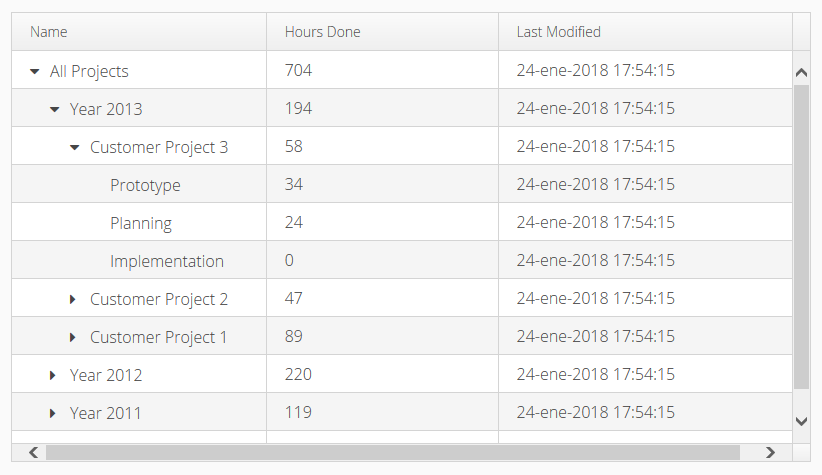
\includegraphics[width=\linewidth]{vaadinExampleImage.png}
	\caption{Árbol de Proyectos}
	\label{fig:vaadinExampleImage}
\end{figure}

\begin{figure}[!tb]
	\centering
	\begin{lstlisting}[language=Java]
	@Override
	protected void init(VaadinRequest request) {
	
	final VerticalLayout layout = new VerticalLayout();
	layout.setSpacing(true);
	layout.setMargin(true);
	
	final TreeGrid grid = new TreeGrid();
	grid.setWidth(800, Unit.PIXELS);
	grid.setHeight(450, Unit.PIXELS);
	
	JobContainer container = new JobContainer();
	grid.setContainerDataSource(container);
	
	layout.addComponent(grid);
	setContent(layout);
	}
	\end{lstlisting}
	\vspace{-15pt}
	\caption{Interfaz de Usuario Vaadin}
	\label{fig:uiVaadin}
\end{figure}

La Figura~\ref{fig:vaadinExampleImage} muestra la interfaz de una pequeña aplicación web consistente en un árbol de tareas. Para construir este ejemplo en \emph{Vaadin}, en primer lugar definimos su interfaz gráfica. Para crear dicha interfaz gráfica, nos basamos en un componente gráfico, o \emph{widget}, denominado \emph{TreeGrid}  (Figura~\ref{fig:jobContainer}, Línea 8). Como puede observarse, este componente gráfico se usa directamente desde código Java, tal como se crearía una interfaz Java de escritorio, utilizando elementos propios de Java como los \emph{layouts} (Figura~\ref{fig:uiVaadin}, Líneas~4\-6) y no siendo necesario escribir nada en Javascript o HTML. Este componente mostrará los datos proporcionados por el contenedor de datos \emph{JobContainer} (Figura~\ref{fig:uiVaadin}, Líneas~12-13).

La clase \emph{JobContainer} (Figura~\ref{fig:jobContainer}) es la que proporcionará los datos que se muestran en el \emph{grid}. Esta clase extiende de una clase de Vaadin llamada \emph{HierarchicalContainer} y se encarga de implementar toda la lógica para almacenar de forma jerárquica los nodos. Además, implementa las interfaces de Vaadin \emph{Collapsible} (Figura~\ref{fig:jobContainerCollapsible}) y \emph{Measurable} (Figura~\ref{fig:jobContainerMeasurable}), encargadas de contraer el árbol de elementos y de calcular la profundidad del elemento en la jerarquía, respectivamente.

\begin{figure}[!tb]
	\centering
	\begin{lstlisting}[language=Java]
	public class JobContainer extends HierarchicalContainer
                               implements Collapsible, Measurable {
	
		static final String PROPERTY_NAME = "Name";
		static final String PROPERTY_HOURS = "Hours done";
		static final String PROPERTY_MODIFIED = "Last modified";
		
		public JobContainer() {
			addContainerProperty(PROPERTY_NAME, String.class, "");
			addContainerProperty(PROPERTY_HOURS, Integer.class, 0);
			addContainerProperty(PROPERTY_MODIFIED, Date.class, new Date());
			
			...	
		}
		
		private Object addItem(Object[] values) {...}
		private Object addChild(Object[] values, Object parentId) {...}
		private void setProperties(Item item, Object[] values) {...}
		private void addChildren(Object itemId) {...}
		private boolean removeChildrenRecursively(Object itemId) {...}
		
		@Override
		public boolean hasChildren(Object itemId) {...}
	}
    \end{lstlisting}
	\caption{Contenedor TreeGrid}
	\label{fig:jobContainer}
\end{figure}


\begin{figure}[!tb]
	\centering
	\begin{lstlisting}[language=Java]
	public class JobContainer
		...
		private Map<Object, Boolean> expandedNodes = new HashMap<>();
			
		@Override
		public void setCollapsed(Object itemId, boolean collapsed) {
			expandedNodes.put(itemId, !collapsed);	
			if (collapsed) {
				removeChildrenRecursively(itemId);
			} else {
				addChildren(itemId);
			}
		}
		
		@Override
		public boolean isCollapsed(Object itemId) {
			return !Boolean.TRUE.equals(expandedNodes.get(itemId));
		}
	}\end{lstlisting}
	\caption{Contenedor TreeGrid Collapsible}
	\label{fig:jobContainerCollapsible}
\end{figure}

\begin{figure}[!tb]
	\centering
	\begin{lstlisting}[language=Java]	
	public class JobContainer
	
		...
		@Override
		public int getDepth(Object itemId) {
			int depth = 0;
			while (!isRoot(itemId)) {
				depth ++;
				itemId = getParent(itemId);
			}
			return depth;
		}
	}\end{lstlisting}
	\caption{Contenedor TreeGrid Measurable}
	\label{fig:jobContainerMeasurable}
\end{figure}

Tal como se puede apreciar, no es necesario ningún conocimiento de las tecnologías web tales como \emph{HTML}, \emph{CSS}, \emph{Javascript}, \emph{HTTP} o \emph{AJAX} para construir el ejemplo de la Figura~\ref{fig:vaadinExampleImage} utilizando \emph{Vaadin}.

\subsection{Arquitectura Interna de \emph{Vaadin}}

Las clases descritas en el apartado anterior se transforman, utilizando \emph{Vaadin}, en código \emph{HTML}, \emph{Javascript} y \emph{CSS} que pueda ser procesado en un navegador web, más una serie de llamadas \emph{AJAX} a una serie de funciones desplegadas en el servidor que se encargan de gestionar la interacción con el servidor, de acuerdo al patrón \emph{Model-View-Presenter (MVP)} (ver Sección~\ref{sec:mvp}). La Figura~\ref{fig:vaadinMVP} muestra el funcionamiento general de este esquema.

\begin{figure}[!tb]
	\centering
	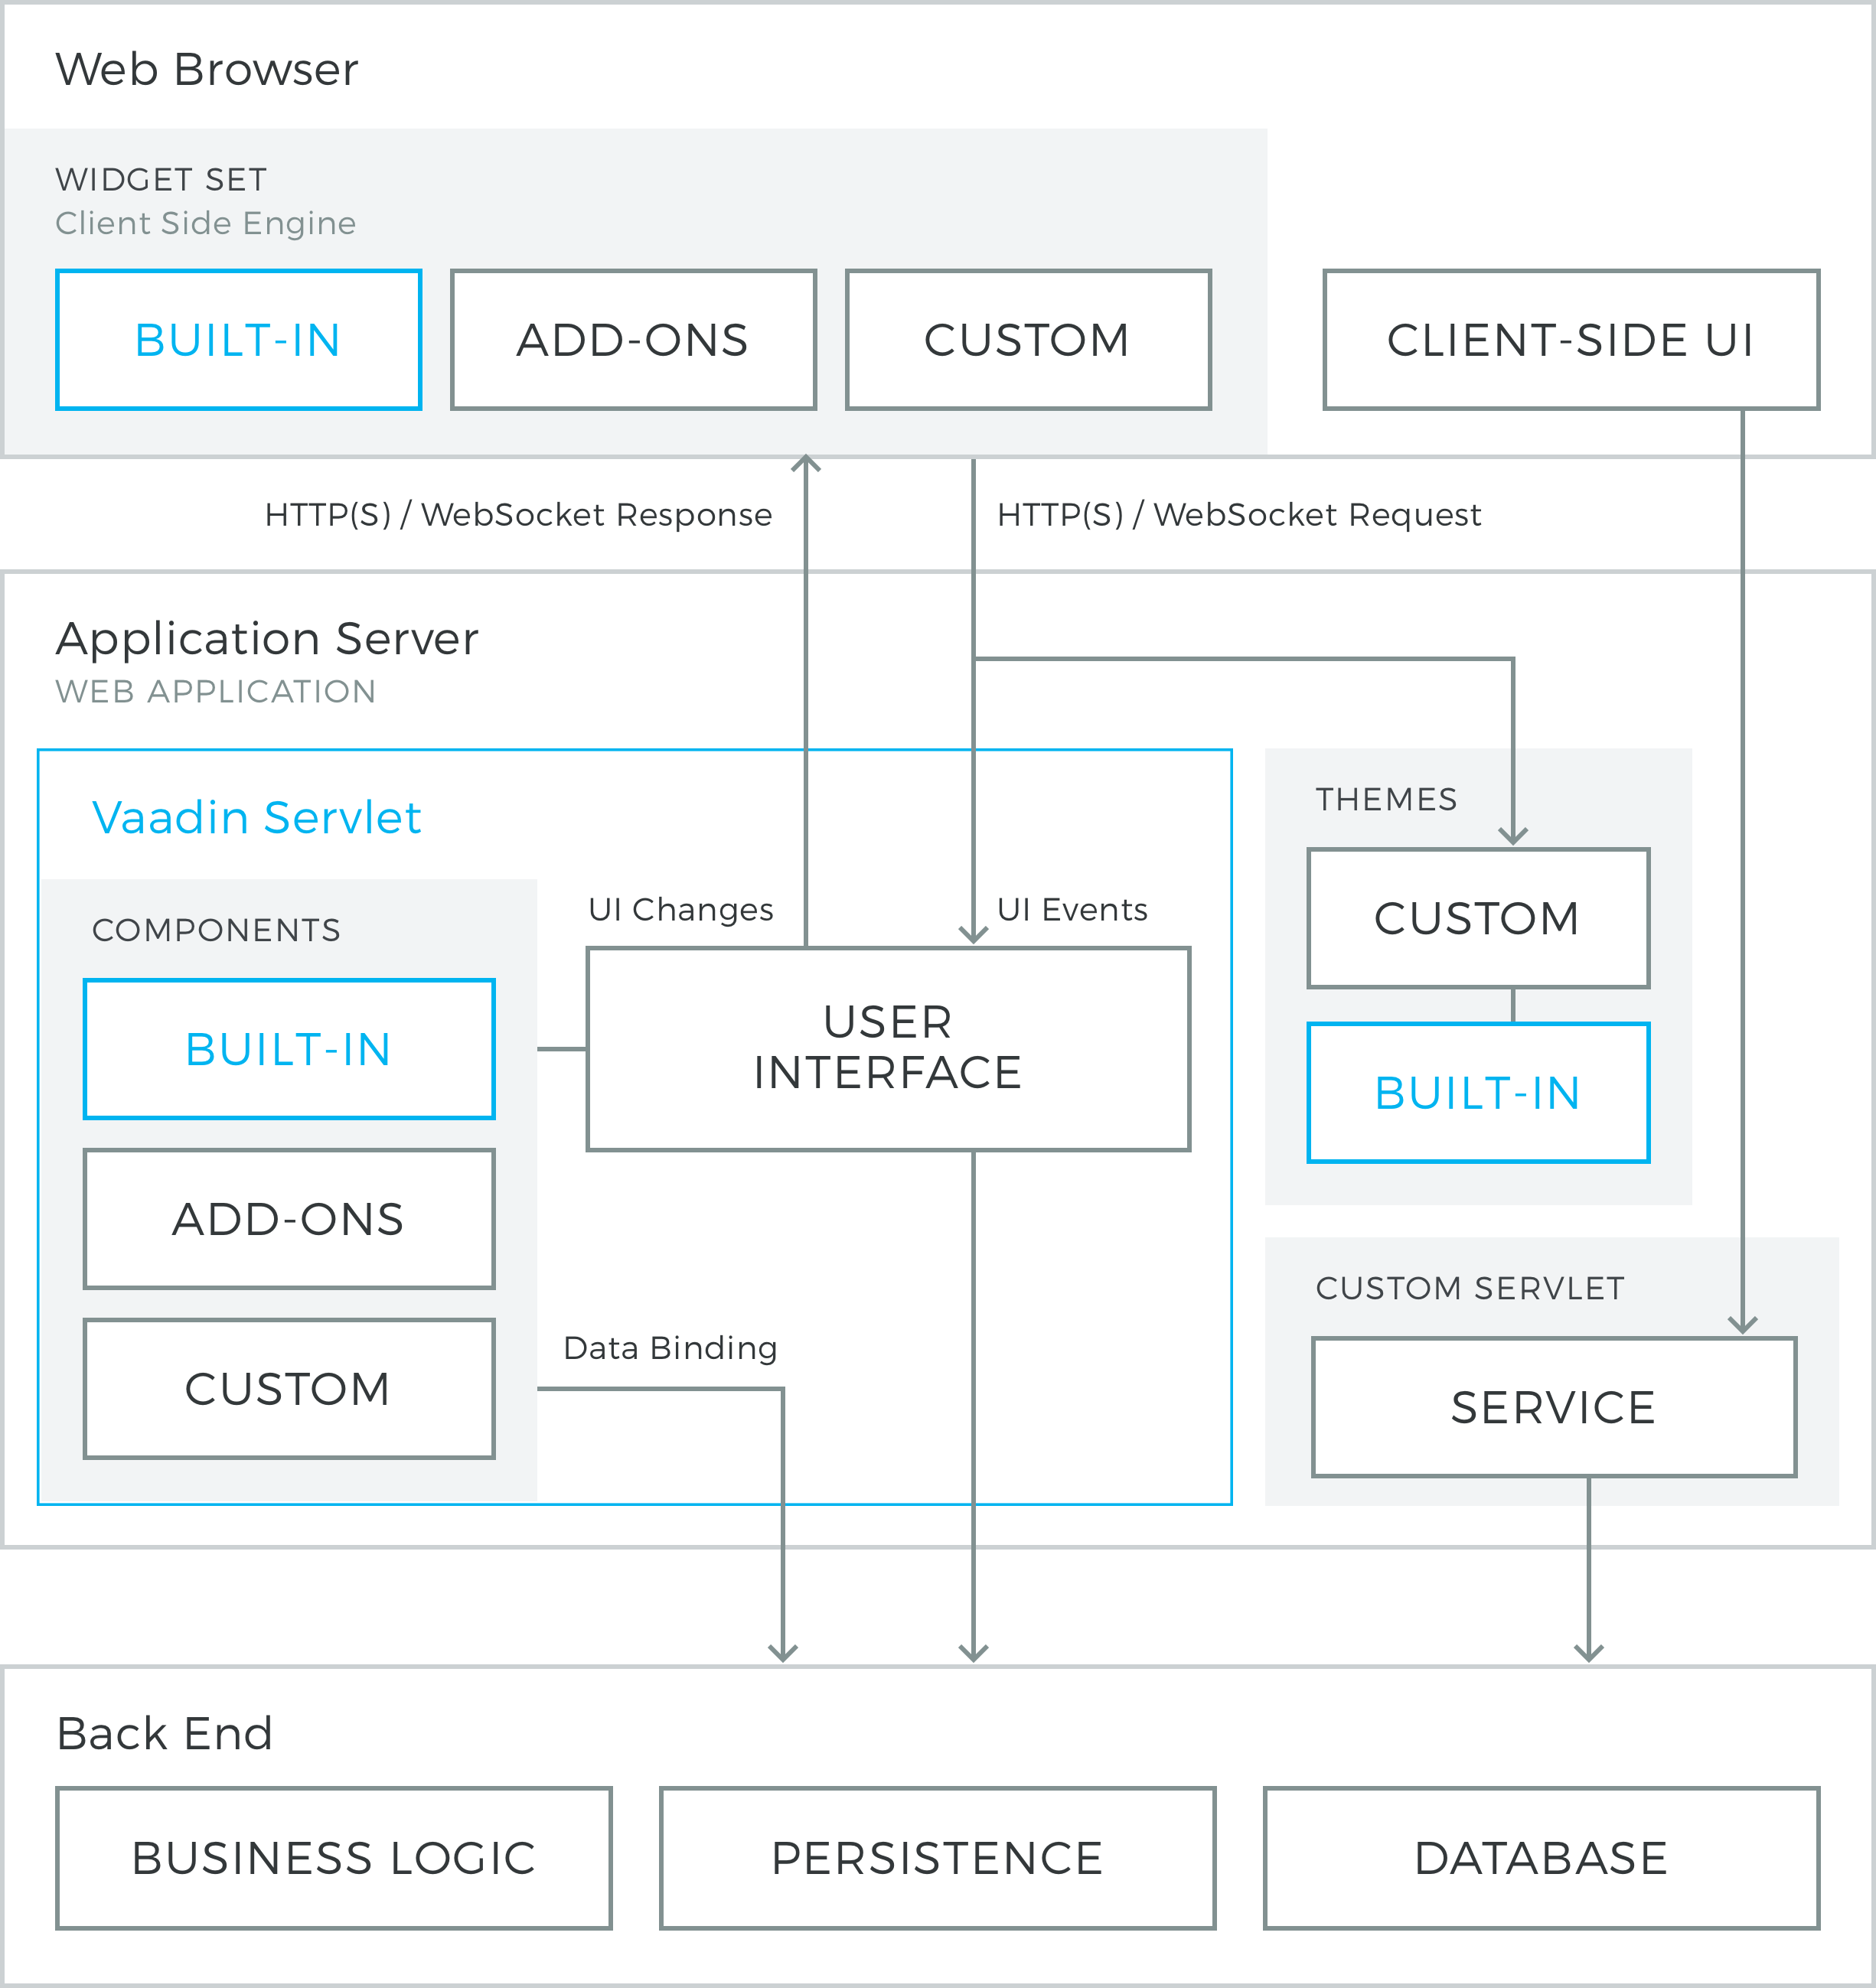
\includegraphics[width=0.80\linewidth]{vaadin/vaadinArch.png}
	\caption{Esquema Modelo-Vista-Presentador en Vaadin}
	\label{fig:fig:vaadinMVP}
\end{figure}

Tal como se puede observar en la Figura~\ref{fig:vaadinMVP}, el código generado por \emph{Vaadin} se estructura en tres módulos: (1) \emph{WebBrowser}; (2) \emph{Back End}; y, (2) \emph{Application Server}.

El primer módulo, \emph{Web Browser}, es el que correría en el lado del cliente y contiene simplemente los elementos necesarios para mostrar los controles gráficos avanzados, recoger los eventos de usuario y comunicarse con el servidor de la aplicación. Este módulo ejerce de \emph{Vista}.

El segundo módulo, \emph{Back End} es el que contiene la lógica de negocio de la aplicación, incluyendo objetos de negocio y la infraestructrura necesaria para persistirlos en bases de datos. Este módulo ejerce de \emph{Modelo}.

El tercer módulo, \emph{Application Server}, es el que hace de puente entre la vista y el modelo, recibiendo los eventos que se realizan sobre la interfaz de usuario y respondiendo de manera adecuada. Este módulo ejerce de \emph{Presentador}.

Cada evento (\emph{UI Events} en Figura~\ref{fig:vaadinMVP}) realizado sobre la interfaz de usuario (\emph{Web Browser}) se delega mediante una petición \emph{AJAX} sobre \emph{HTTP} al módulo \emph{Application Server}. Este módulo es el que decide cómo la aplicación debe reaccionar a dicho evento. Esta reacción podría implicar desde simple cambio en la interfaz gráfica hasta el procesamiento de una larga y compleja regla de negocio. 

Por ejemplo, si se decide desplegar un año dentro del árbol de tareas de la Figura~\ref{fig:vaadinExampleImage}, este evento se delega en la capa de aplicación (\emph{Application Server}), que devuelve los datos necesarios, para actualizar la interfaz gráfica. Si, por otro lado, quisiéramos añadir una nueva tarea a nuestro árbol de tareas, este evento se delegaría de nuevo en la capa de aplicación, la cual llamaría a la parte de negocio (\emph{Back End}) para iniciar una transacción que, tras verificar que se puede añadir dicha tarea de acuerdo con las reglas definidas para el negocio, actualice el estado de los objetos de negocio de manera adecuada, y los refleje en la base de datos correspondiente. 

%%================================================================================%%
%% NOTe(Pablo): Suprimido                                                         %%
%%================================================================================%%
%%
%% Ambos módulos se comunican entre si a partir de \emph{APIs}\cite{api} propias, 
%% y tienen un modelo de componentes y elementos gráficos copia en ambos lados. 
%% De este modo si se produce un evento sobre la interfaz, el lado cliente se 
%% comunica con la \emph{API} servidora para notificarla los eventos y/o los 
%% cambios en los componentes, una vez recibida y tratada la llamada en el lado
%% servidor, este se encarga de conectarse a la \emph{API} cliente junto con los 
%% nuevos componentes gráficos, es decir, la nueva vista, para que el lado 
%% cliente la muestre por pantalla.
%%
%%
%% A raíz de este comportamiento, Vaadin suele estar ligado al patrón 
%% \emph{MVP}\cite{mvp} (explicado en el apartado de la arquitectura de LUCA) 
%% debido a que aísla la vista del modelo y las conecta a través de un 
%% intermediario que es el presentador, este se encarga de comunicarse con ambas 
%% y de ejecutar la lógica de negocio de la aplicación. De este modo cuando en 
%% la vista se produce un cambio, es notificado en el presenter, este lo gestiona
%%  (comunicándose con el modelo si es necesario) y después manda a la vista 
%% recargarse con los cambios producidos. Se puede apreciar que siguiendo este 
%% patrón, el conjunto de componentes que proporciona la vista para mostrar por 
%% pantalla estarían de forma duplicada tanto en la parte servidora como cliente 
%% a espera de recibir eventos o ser recargadas.
%%
%%==========================================================================%%
%% NOTA(Pablo): Decir esto y no decir nada es lo mismo. Te lo he encauzado  %%
%%    un poco mejor arriba.                                                 %%
%%==========================================================================%%
%%
%% Echando un breve vistazo a la interacción cliente/servidor que facilita
%%  Vaadin, podemos explicar el código desde un punto de vista cliente y
%% servidor. El navegador, que realiza las funciones de cliente, recibe el
%% conjunto de ficheros \emph{HTML},\emph{Javascript} y \emph{CSS}
%% necesarios para formar la vista, este lado se encarga de cargar y
%% visualizar dichos ficheros, así como, de recibir las acciones sobre la
%% vista para comunicarlas a la parte servidora, utilizando para ello
%% llamadas \emph{AJAX}\cite{ajax}. Desde el punto de vista servidor,
%% Vaadin recibe las llamadas y las trata para posteriormente recargar
%% la vista enviando una respuesta al cliente.
%%
%% Extrapolando al ejemplo, la \emph{UI} se compilará para poder ser
%% visualizada por un navegador. El usuario al interactuar con la interfaz,
%%  enviará eventos a través del contenedor de datos, una vez finalizados
%% los eventos, se volverá a recargar la vista para hacer visibles los
%%  cambios. De esta forma, en la parte cliente se almacenarán los ficheros
%% \emph{HTML},\emph{Javascript} y \emph{CSS} mientras que en la parte
%% servidora se encontrará toda la lógica.
%%
%%==========================================================================%%
%%
%% Con estas indicaciones se ha creado un ejemplo sencillo de composición de 
%% elementos jerárquicos entre sí utilizando Vaadin, como podemos ver ha 
%% facilitado mucho su implementación respecto a una configuración basada en
%%  \emph{HTML} o \emph{Javascript}.
%% 
%%==========================================================================%%

